\let\negmedspace\undefined
\let\negthickspace\undefined
\documentclass[journal]{IEEEtran}
\usepackage{adjustbox}
\usepackage[a5paper, margin=10mm, onecolumn]{geometry}
\usepackage{tfrupee} % Include tfrupee package
\usepackage{gvv-book}
\usepackage{gvv}
\usepackage{cite}
\usepackage{amsmath,amssymb,amsfonts,amsthm}
\usepackage{algorithmic}
\usepackage{graphicx}
\usepackage{textcomp}
\usepackage{xcolor}
\usepackage{txfonts}
\usepackage{listings}
\usepackage{enumitem}
\usepackage{mathtools}
\usepackage{gensymb}
\usepackage{comment}
\usepackage[breaklinks=true]{hyperref}
\usepackage{tkz-euclide}
\usepackage{array}
\usepackage{longtable}
\usepackage{calc}
\usepackage{multirow}
\usepackage{hhline}
\usepackage{ifthen}
\usepackage{lscape}
 \usepackage{booktabs}
\usepackage{fancyhdr}
\usepackage{float}
\usepackage{tikz}
\usetikzlibrary{positioning, shapes.geometric, arrows}

\setlength{\headheight}{1cm}
\setlength{\headsep}{0mm}

\pagestyle{fancy}
\fancyhf{}
\fancyhead[L]{\leftmark}
\fancyhead[R]{\thepage}

\renewcommand{\thefigure}{\theenumi}
\renewcommand{\thetable}{\theenumi}
\setlength{\intextsep}{10pt}

\numberwithin{equation}{enumi}
\numberwithin{figure}{enumi}
\renewcommand{\thetable}{\theenumi}

\title{HARDWARE ASSIGNMENT}
\author{EE24BTECH11029-SHRETHAN REDDY}
\date{\today}

\begin{document}

\maketitle

\tableofcontents
\newpage

\section{Introduction}
This document provides a step-by-step procedure for creating a digital clock using an IC 7447 (BCD to 7-segment decoder) and an Arduino. The circuit involves interfacing the Arduino with the IC to drive a 7-segment display.
\section{Materials Required}
\begin{table}[h]
    \centering
    \begin{tabular}{|c|c|c|}
        \hline
        \textbf{Component} & \textbf{Quantity} & \textbf{Purpose and Connection} \\
        \hline
        Arduino Uno & 1 & Main microcontroller unit \\
        7447 Decoder & 1 & Converts BCD to 7-segment display signals \\
        Common Anode 7-Segment Display & 6 & Displays time digits \\
        220$\Omega$ Resistors & 6 & Current limiting resistors for displays \\
        % Push Buttons & 3 & Used for manual hour, minute, and second adjustments \\
        Breadboards & 2 & For making connections \\
        Jumper Wires & Multiple & For electrical connections \\
        \hline
    \end{tabular}
    \caption{List of components and their usage}
    \label{tab:components}
\end{table}
\section{Circuit Connections}
\subsection{Connecting Arduino to IC 7447}
\begin{itemize}
    \item Connect Arduino digital pins (e.g., D2, D3, D4, D5) to the BCD input pins of IC 7447 (pins 7, 1, 2, 6).
    \item These pins will send the BCD (Binary Coded Decimal) data to the IC.
\end{itemize}
\begin{table}[h!]
\centering
\begin{tabular}{|c|c|c|}
\hline
\textbf{IC 7447 Pin} & \textbf{Arduino Pin} & \textbf{Description} \\
\hline
Pin 7 (A) & D2 & BCD Input (LSB) \\
Pin 1 (B) & D3 & BCD Input \\
Pin 2 (C) & D4 & BCD Input \\
Pin 6 (D) & D5 & BCD Input (MSB) \\
Pin 16 (VCC) & 5V & Power Supply \\
Pin 8 (GND) & GND & Ground \\
\hline
\end{tabular}
\caption{IC 7447 to Arduino Pin Connections}
\end{table}
\begin{tikzpicture}[
    box/.style={draw, rectangle, rounded corners, minimum width=2.5cm, minimum height=1cm, text centered, font=\bfseries},
    arrow/.style={->, >=stealth', thick, shorten <=1pt, shorten >=1pt},
    pin/.style={font=\small}
]

    % Nodes
    \node[box, fill=blue!20] (arduino) {Arduino};
    \node[pin, below=0.2cm of arduino] (arduinoLabel) {Digital Pins};

    \node[box, fill=green!20, right=2cm of arduino] (ic7447) {IC 7447};
    \node[pin, below=0.2cm of ic7447] (icLabel) {BCD Inputs};

    \node[box, fill=red!20, right=2cm of ic7447] (display) {7-Segment Display};
    \node[pin, below=0.2cm of display] (displayLabel) {Segments (a-g)};

    % Power Supply
    \node[box, fill=yellow!20, below=1.5cm of ic7447] (power) {Power Supply};

    % Arduino to IC 7447 Connections
    \draw[arrow] ([yshift=0.4cm]arduino.east) -- node[above] {D2 (A)} ([yshift=0.4cm]ic7447.west);
    \draw[arrow] ([yshift=0.1cm]arduino.east) -- node[above] {D3 (B)} ([yshift=0.1cm]ic7447.west);
    \draw[arrow] ([yshift=-0.2cm]arduino.east) -- node[above] {D4 (C)} ([yshift=-0.2cm]ic7447.west);
    \draw[arrow] ([yshift=-0.5cm]arduino.east) -- node[above] {D5 (D)} ([yshift=-0.5cm]ic7447.west);

    % IC 7447 to 7-Segment Display Connections
    \foreach \y/\label in {0.4/a, 0.2/b, 0/c, -0.2/d, -0.4/e, -0.6/f, -0.8/g} {
        \draw[arrow] ([yshift=\y cm]ic7447.east) -- node[above] {\label} ([yshift=\y cm]display.west);
    }

    % Power and Ground Connections
    \draw[arrow] (power.north) -- ++(0, 0.4) -| ([yshift=-0.8cm]ic7447.south) node[midway, above] {VCC (5V)};
    \draw[arrow] ([yshift=-0.8cm]ic7447.south) -- ++(0, -0.4) node[below] {GND};

\end{tikzpicture}
\newpage
\subsection{Connecting IC 7447 to the 7-Segment Display}
\begin{itemize}
    \item Connect the output pins of IC 7447 (pins 9, 10, 11, 12, 13, 14, 15) to the corresponding segments (a, b, c, d, e, f, g) of the 7-segment display.
    \item Use $220\Omega$ resistors between the IC outputs and the display segments to limit current.
\end{itemize}

\subsection{Powering the IC and Display}
\begin{itemize}
    \item Connect the VCC (pin 16) of IC 7447 to the 5V pin of the Arduino.
    \item Connect the GND (pin 8) of IC 7447 to the GND of the Arduino.
    \item Connect the common cathode of the 7-segment display to GND.
\end{itemize}

\subsection{Optional: Adding Push Buttons for Time Setting}
\begin{itemize}
    \item Connect push buttons to Arduino digital pins (e.g., D6, D7) for incrementing hours and minutes.
    \item Use pull-down resistors $(10k\Omega)$ for each button.
\end{itemize}

\begin{figure}[H]
    \centering
    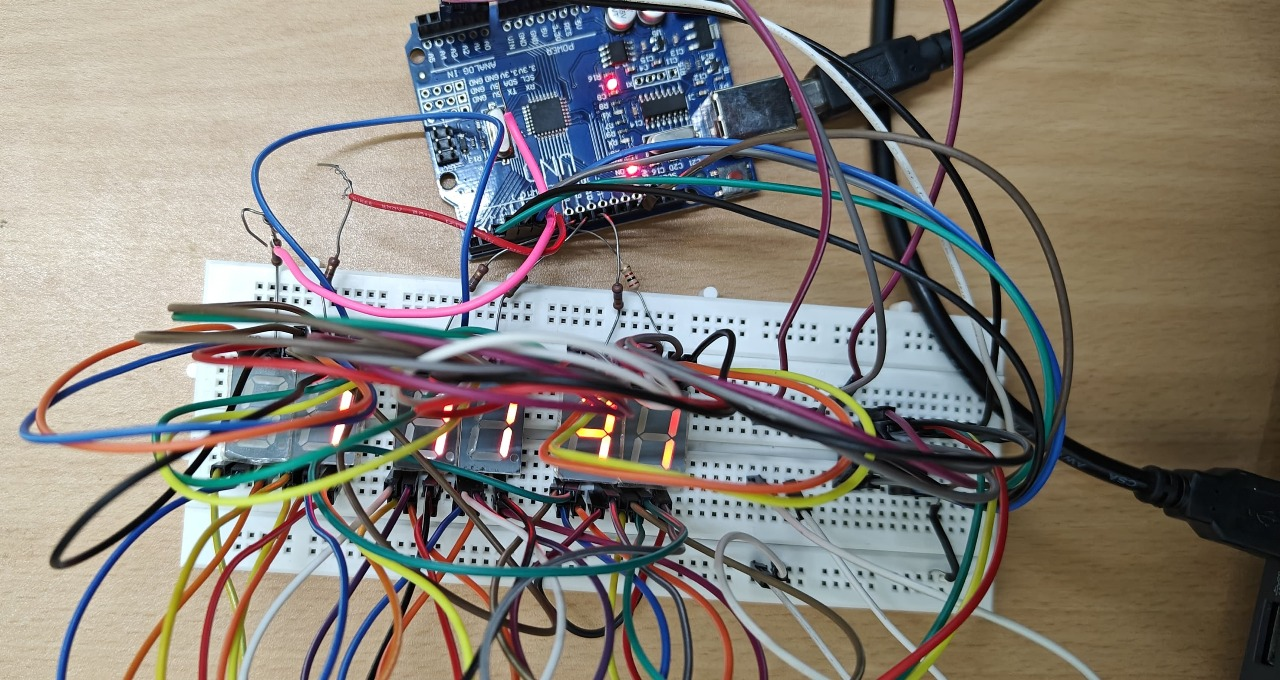
\includegraphics[width=0.8\linewidth]{figure/fig1.png}
    \caption{Circuit Diagram}
    \label{fig:circuit}
\end{figure}

\section{Arduino Code}
Upload the following code to the Arduino:

\begin{lstlisting}[language=C++, caption={Arduino Code for Clock}, basicstyle=\ttfamily\footnotesize, keywordstyle=\color{blue}, commentstyle=\color{green}, numbers=left, numberstyle=\tiny\color{gray}]
// Define BCD output pins
#include <avr/io.h>
#include <avr/interrupt.h>
#include <util/delay.h>

// BCD Output Pins
#define A PD2
#define B PD3
#define C PD4
#define D PD5

// Common Display Pins
#define H1 PD6
#define H2 PD7
#define M1 PB0
#define M2 PB1
#define S1 PB2
#define S2 PB3

// Button Pins
#define SET_HOUR PC1
#define SET_MIN PC2
#define SET_SEC PC0
#define RESET_BTN PC3

// Global BCD digits for the clock
volatile uint8_t h1 = 0, h2 = 0, m1 = 0, m2 = 0, s1 = 0, s2 = 0;

// Multiplexing control variables
uint8_t current_digit = 0;
volatile uint32_t millis_count = 0;
const uint8_t mux_interval = 2; // 2ms per digit refresh

// Timekeeping control
volatile uint32_t last_second = 0;

// Button debouncing
volatile uint32_t last_button_check = 0;
const uint16_t debounce_interval = 200;

void init_timer0() {
    TCCR0A |= (1 << WGM01);
    TCCR0B |= (1 << CS01) | (1 << CS00);
    OCR0A = 249;
    TIMSK0 |= (1 << OCIE0A);
    sei();
}

ISR(TIMER0_COMPA_vect) {
    millis_count++;
}

uint32_t millis() {
    uint32_t ms;
    cli();
    ms = millis_count;
    sei();
    return ms;
}

uint8_t bcdIncrement(uint8_t bcd, uint8_t max) {
    if (bcd == max) return 0;
    uint8_t d0 = bcd & 0x01, d1 = (bcd >> 1) & 0x01, d2 = (bcd >> 2) & 0x01, d3 = (bcd >> 3) & 0x01;
    uint8_t n0 = !d0, c0 = d0, n1 = d1 ^ c0, c1 = d1 & c0, n2 = d2 ^ c1, c2 = d2 & c1, n3 = d3 ^ c2;
    return (n3 << 3) | (n2 << 2) | (n1 << 1) | n0;
}

void reset_time() {
    cli();
    h1 = h2 = m1 = m2 = s1 = s2 = 0;
    last_second = millis();
    sei();
}

void updateTime() {
    if (millis() - last_second >= 1000) {
        last_second += 1000;
        s2 = bcdIncrement(s2, 9);
        if (s2 == 0) {
            s1 = bcdIncrement(s1, 5);
            if (s1 == 0) {
                m2 = bcdIncrement(m2, 9);
                if (m2 == 0) {
                    m1 = bcdIncrement(m1, 5);
                    if (m1 == 0) {
                        h2 = bcdIncrement(h2, 9);
                        if (h2 == 0) {
                            h1 = bcdIncrement(h1, 2);
                            if (h1 == 2 && h2 > 3) {
                                h1 = h2 = 0;
                            }
                        }
                    }
                }
            }
        }
    }
}

void set_time() {
    if (millis() - last_button_check > debounce_interval) {
        if (!(PINC & (1 << SET_HOUR))) {
            h2 = bcdIncrement(h2, 9);
            if (h2 == 0) h1 = bcdIncrement(h1, 2);
            if (h1 == 2 && h2 > 3) {
                h1 = h2 = 0;
            }
            last_button_check = millis();
        }
        if (!(PINC & (1 << SET_MIN))) {
            m2 = bcdIncrement(m2, 9);
            if (m2 == 0) m1 = bcdIncrement(m1, 5);
            last_button_check = millis();
        }
        if (!(PINC & (1 << SET_SEC))) {
            s2 = bcdIncrement(s2, 9);
            if (s2 == 0) s1 = bcdIncrement(s1, 5);
            last_button_check = millis();
        }
        if (!(PINC & (1 << RESET_BTN))) {
            reset_time();
            last_button_check = millis();
        }
    }
}

void displayDigit(uint8_t digit, uint8_t position) {
    PORTD &= ~((1 << H1) | (1 << H2));
    PORTB &= ~((1 << M1) | (1 << M2) | (1 << S1) | (1 << S2));
    
    PORTD &= ~((1 << A) | (1 << B) | (1 << C) | (1 << D));
    PORTD |= ((digit & 0x01) << A) |
             ((digit & 0x02) << (B-1)) |
             ((digit & 0x04) << (C-2)) |
             ((digit & 0x08) << (D-3));
    
    switch (position) {
        case 0: PORTD |= (1 << H1); break;
        case 1: PORTD |= (1 << H2); break;
        case 2: PORTB |= (1 << M1); break;
        case 3: PORTB |= (1 << M2); break;
        case 4: PORTB |= (1 << S1); break;
        case 5: PORTB |= (1 << S2); break;
    }
    
    _delay_ms(mux_interval);
}

void multiplexDisplay() {
    uint8_t digits[6] = {h1, h2, m1, m2, s1, s2};
    displayDigit(digits[current_digit], current_digit);
    current_digit = (current_digit + 1) % 6;
}

void setup() {
    DDRD |= (1 << A) | (1 << B) | (1 << C) | (1 << D) | (1 << H1) | (1 << H2);
    DDRB |= (1 << M1) | (1 << M2) | (1 << S1) | (1 << S2);
    
    DDRC &= ~((1 << SET_HOUR) | (1 << SET_MIN) | (1 << SET_SEC) | (1 << RESET_BTN));
    PORTC |= (1 << SET_HOUR) | (1 << SET_MIN) | (1 << SET_SEC) | (1 << RESET_BTN);
    
    init_timer0();
    
    last_second = millis();
    last_button_check = millis();
}

int main(void) {
    setup();
    
    while (1) {
        set_time();
        updateTime();
        multiplexDisplay();
    }
    
    return 0;
}
\end{lstlisting}

\section{Testing and Calibration}
\begin{itemize}
    \item Upload the code to the Arduino.
    \item Power the circuit and observe the 7-segment display.
    \item If using buttons, press them to adjust the time.
    \item Ensure the display shows the correct time and increments properly.
\end{itemize}

\section{Enhancements}
\begin{itemize}
    \item Add multiple 7-segment displays for hours and minutes.
    \item Use a real-time clock (RTC) module like DS3231 for accurate timekeeping.
    \item Add a colon separator between hours and minutes using an LED.
\end{itemize}

\section{Conclusion}
This setup creates a basic digital clock using IC 7447 and Arduino. It can be expanded further based on specific requirements.


\end{document}
